% CCI v2 -- "hero box" for the headline CFR-reduction result.
% Standalone preview; the same TikZ goes inline into poster.tex Block 6.
\documentclass[tikz,border=10pt]{standalone}
\usepackage{amsmath}
\usepackage{array}
\usepackage{colortbl}

% EPFL palette (already defined in poster.tex; redefined here for standalone)
\definecolor{epflred}{HTML}{B51F1F}
\definecolor{epflcoal}{HTML}{413D3A}
\definecolor{epfllead}{HTML}{707070}

\usetikzlibrary{shadows.blur}

\begin{document}
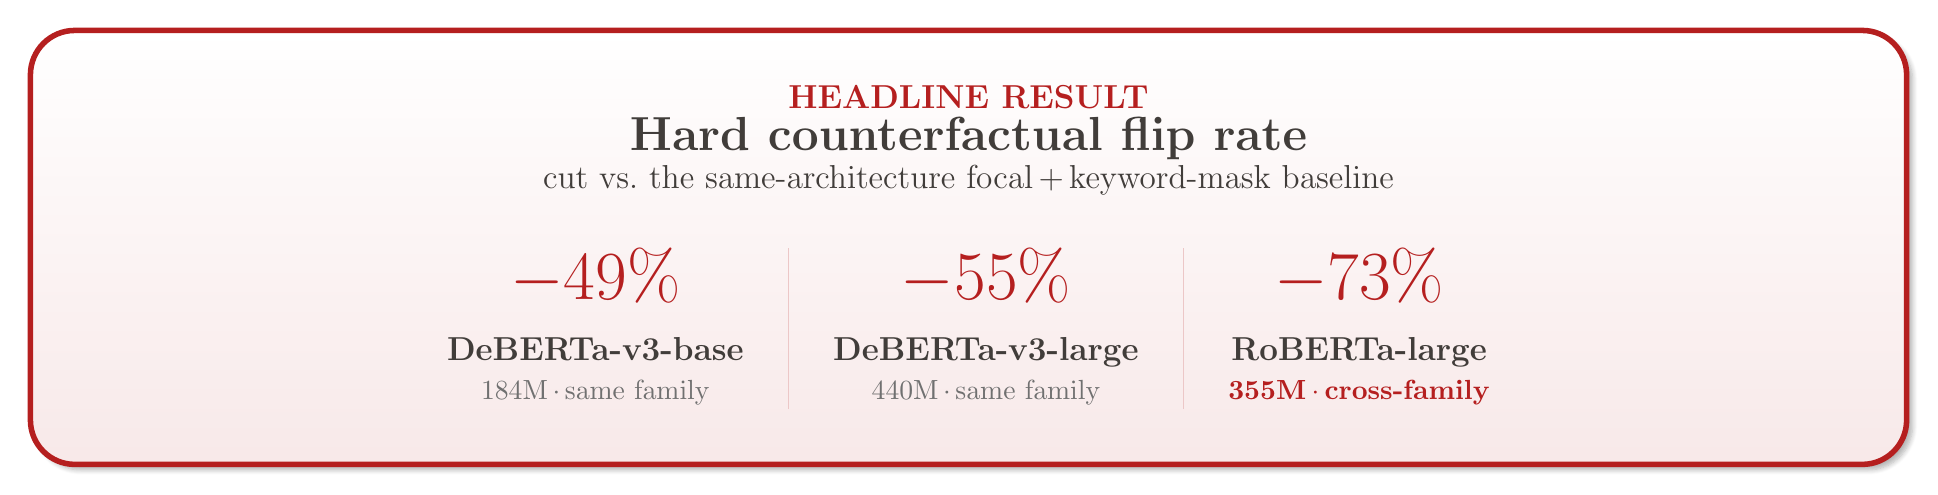
\begin{tikzpicture}
\node[draw=epflred, line width=2pt, rounded corners=16pt,
      top color=white, bottom color=epflred!10,
      inner xsep=26pt, inner ysep=20pt,
      blur shadow={shadow blur steps=7, shadow yshift=-2pt, shadow opacity=30}]
{%
  \begin{minipage}{22cm}\centering
    % eyebrow
    {\color{epflred}\bfseries\large HEADLINE RESULT}\\[3pt]
    % title
    {\color{epflcoal}\LARGE\textbf{Hard counterfactual flip rate}}\\[2pt]
    {\color{epflcoal}\large cut vs.\ the same-architecture focal\,+\,keyword-mask baseline}\\[18pt]
    % the three big numbers, separated by light vertical rules
    \setlength{\arrayrulewidth}{1pt}%
    \begin{tabular}{@{\hspace{4pt}}c@{\hspace{16pt}}
                    !{\color{epflred!25}\vrule}@{\hspace{16pt}}c@{\hspace{16pt}}
                    !{\color{epflred!25}\vrule}@{\hspace{16pt}}c@{\hspace{4pt}}}
      {\color{epflred}\fontsize{66}{66}\selectfont\textbf{$-49\%$}} &
      {\color{epflred}\fontsize{66}{66}\selectfont\textbf{$-55\%$}} &
      {\color{epflred}\fontsize{66}{66}\selectfont\textbf{$-73\%$}} \\[10pt]
      {\color{epflcoal}\large\textbf{DeBERTa-v3-base}} &
      {\color{epflcoal}\large\textbf{DeBERTa-v3-large}} &
      {\color{epflcoal}\large\textbf{RoBERTa-large}} \\[2pt]
      {\color{epfllead} 184M\,$\cdot$\,same family} &
      {\color{epfllead} 440M\,$\cdot$\,same family} &
      {\color{epflred}\textbf{355M\,$\cdot$\,cross-family}} \\
    \end{tabular}
  \end{minipage}%
};
\end{tikzpicture}
\end{document}
